% !TEX TS-program = pdflatex
% !TEX encoding = UTF-8 Unicode
% !BIB TS-program = biber
% !BIB program = biber

\documentclass[12pt]{article}

%%% PAGE DIMENSIONS
\usepackage[margin=2.54cm]{geometry}
\geometry{a4paper} 

\usepackage{graphicx} % For better graphics
\usepackage{pdfpages} % To insert pdfs into the library
\usepackage{tikz}
\usepackage{wrapfig}

%%% PACKAGES
\usepackage{booktabs} % for much better looking tables
\usepackage{amsmath} % for better maths
\usepackage{paralist} % very flexible & customisable lists (eg. enumerate/itemize, etc.)
\usepackage{verbatim} % adds environment for commenting out blocks of text & for better verbatim
\usepackage{subfig} % make it possible to include more than one captioned figure/table in a single float
\usepackage[framed,numbered]{matlab-prettifier} % enable inserting matlab code.
\usepackage[parfill]{parskip}
%\addtolength{\jot}{1em}
\usepackage{amssymb}
\usepackage{cancel}
\usepackage{color}
\usepackage{listings}
\usepackage{multicol}
\usepackage{float}

% References
\usepackage[backend=biber]{biblatex}
\bibliography{sources}

%%% HEADERS & FOOTERS
\usepackage{fancyhdr} % This should be set AFTER setting up the page geometry
\setlength{\headheight}{15pt}
\pagestyle{fancy} % options: empty , plain , fancy
\renewcommand{\headrulewidth}{0pt} % customise the layout...
\lhead{ENGSCI 700AB}\chead{Global Carbon Pricing}\rhead{cmcd398}
\lfoot{}\cfoot{\thepage}\rfoot{}

%%% SECTION TITLE APPEARANCE
\usepackage{sectsty}

%%% ToC (table of contents) APPEARANCE
\usepackage[nottoc,notlof,notlot]{tocbibind} % Put the bibliography in the ToC
\usepackage[titles,subfigure]{tocloft} % Alter the style of the Table of Contents
\renewcommand{\cftsecfont}{\rmfamily\mdseries\upshape}
\renewcommand{\cftsecpagefont}{\rmfamily\mdseries\upshape} % No bold!

%%% Hyperlinking 
\usepackage{hyperref}
\begin{document}
\begin{titlepage}
	\newcommand{\HRule}{\rule{\linewidth}{0.5mm}} % Defines a new command for horizontal lines, change thickness here
	
	\center
	
	%------------------------------------------------
	%	Headings
	%------------------------------------------------
	
	\textsc{\LARGE }\\[1.5cm] % Main heading such as the name of your university/college
	
	\textsc{\Large ENGSCI 700A/B}\\[0.5cm] % Major heading such as course name
	
	%------------------------------------------------
	%	Title
	%------------------------------------------------
	
	\HRule\\[0.5cm]
	
	{\huge\bfseries ENGSCI 700 Research}\\[0.4cm] % Title of your document
	
	\HRule\\[0.5cm]
	
	%------------------------------------------------
	%	Author(s)
	%------------------------------------------------
	
	{\large\textit{Connor McDowall \\cmcd398 \\530913386}}\\
	
	%------------------------------------------------
	%	Date
	%------------------------------------------------
	
	\vfill\vfill\vfill % Position the date 3/4 down the remaining page
	
	{\large\today} % Date, change the \today to a set date if you want to be precise
	 
	%----------------------------------------------------------------------------------------
	
	\vfill % Push the date up 1/4 of the remaining page
	
\end{titlepage}
\lstlistoflistings
\tableofcontents
\listoffigures
\listoftables

\newpage


\section{Journal Log and Supervisor Meetings}
\subsection{Meeting 1: 19/03/18 in Person}
Discussion Points
    \begin{itemize}
        \item COVID-19: Planning to move University and Project Online
        \item COVID-19: Impact on Share Prices
        \item Eyal Ofer and Stock Market Volitility
        \item Commtrade.co.nz and NZ Carbon Price Spot Market
    \end{itemize}
Action Points
    \begin{itemize}
        \item Waka and Kayak Energy Scenarios
        \item Emissions Trading Scheme
        \item Economic Model underpinning the Scenarios
    \end{itemize}
    \subsection{Meeting 2: 25/03/18 via Zoom}
Discussion Points
    \begin{itemize}
        \item Relocation around the Country
        \item Outline of existing research document
        \item Discussed meeting
    \end{itemize}
Action Points
    \begin{itemize}
        \item Continue with Research Document
        \item Looks at wider socio-economic factors
        \item Understand TIME and MARKAL Model
        \item John Carnegie is now head of PEPANZ. Rosalind 
              mentioned getting coffee with him when COVID-19
              lockdown finishes.
    \end{itemize}
\subsection{Meeting 3: 9/04/18 via Zoom}
Discussion Points
    \begin{itemize}
        \item Meeting postponed 
    \end{itemize}
Action Points
    \begin{itemize}
        \item Insert
    \end{itemize}

\subsection{Meeting 4: 16/04/18 via Zoom}
    Discussion Points
        \begin{itemize}
            \item COVID-19 Response from Auckland and Victoria
            \item Research resources
            \item Discussion on getting GAMS on FlexIT
        \end{itemize}
    Action Points
        \begin{itemize}
            \item Continue research document and drafting literature review
            \item Test FlexIT System when access granted
        \end{itemize}
\subsection{Meeting 5: 23/04/20 via Zoom}
Progress Report (16/04/20 - 23/04/20)
\begin{itemize}
    \item Drafted two of five pages for literature review
    \item Reviewed twelve academic papers/journals/reports for Literature Review
\end{itemize}
Discussion Points
    \begin{itemize}
        \item Oil Market Activity including WTI Negative Oil Prices
        \item Rosalind's experience at Stanford (Alumni Commitments, PHD, Computer Science Course)
        \item Installing a VM in install GAMS
        \item Quality of Literature and Reliable Sources
    \end{itemize}
Action Points
    \begin{itemize}
        \item Continue research document and drafting literature review to submit to Rosalind on 27th of April
        \item Test FlexIT System when access granted
    \end{itemize}
    \subsection{Meeting 6: 30/04/20 via Zoom}
Progress Report (23/04/20 - 30/04/20)
\begin{itemize}
    \item Drafted eight of 10 pages for literature review
    \item Reviewed 26 academic papers/journals/reports for Literature Review
    \item 
\end{itemize}
Discussion Points
    \begin{itemize}
        \item 
    \end{itemize}
Action Points
    \begin{itemize}
        \item 
    \end{itemize}






    \section{New Zealand Energy Scenarios}
    \begin{itemize}
        \item   The report informs how to leverage New Zealand's competitive advantage
                with abundant natural resources, ease of business, strong export sector
                and high standards of to inform how we sustainably grow business while
                addressing the issues in the global energy sector.
        \item   Predicting the future becomes harder with technological development,
                requirements for quicker policy changes, and investment decisions.
        \item   The BusinessNZ Energy Council has developed a report outlining two different
                future energy scenarios for New Zealand (Kayak and Waka)
        \item   19 critical uncertainties underpin these two scenarios. These varied from 
                external sources such as \textbf{global stability}, domestic economy factors
                such as \textbf{International Fuel Markets, urban sustainability, energy affordability
                , and the allocation of natural resources} 
        \item   The world energy council (WEC) is the principal impartial network of energy
                leaders (3000 member organisations in 100 Counntries) to plan these scernarios.
        \item   The scenarios enable businesses and policy makers to make decisions to inform
                their future strategy and operations.
        \item   The scenarios are to: develop a platform for ongoing projects and researching 
                energy options for New Zealand’s future create a positive policy and investment 
                climate that promotes new technology and innovation, as well as supporting energy 
                sector developments.
    \end{itemize}
    \subsection{Kayak Scenario}
    \begin{itemize}
        \item   The markets drive supply chain decisions and innovation more than the government.
                Consumers and Producers will make decisions in their best interests based on price
                and quantity. Market forces drvei the decisions. The government focuses on
                establishing strong competitive frameworks relying on the pursuit of least
                cost energy supply. International commitments to reducing emissions are weak.
        \item   The government relies on net immigration and the public perception of New Zealand being
                being clean and green.
        \item   Heightened environmental awareness will drive businesses and consumers to rely on GOVT to make
                decisions in national interest. Markets and technology deliver more affordable energy over time
                with a greater focus on energy equity. There will be no support for low-carbon technologies
                apart from a modest carbon price. 
        \item   Key statistics in 2050:6.15m population, 503B GDP, \$ 60 / Tonne. ~30 Mt/pa of Carbon Emissions.
                85\% of electricity generated from renewable resources. Greater focus on energy equity over security
                and sustainability. No change in energy intensity per annum.
    
    \end{itemize}
    \subsection{Waka Scenario}
    \begin{itemize}
        \item   Business and Consumers reply on Government to make decisions from a nationalist perspective
                to meet environmental sustainability goals.
        \item   Reducing global carbon emissions will be at the expense of economic growth. Exports will be
                be hurt by rising global carbon prices. New Zealand loses it's competitive advantage with a 
                sustainable green image.
        \item   New Zealand focuses on disrupting traditional methods of transport and adopting 100\% 
                renewables for electricity generation (Confirm if Retail and/or Industrial Demand).
        \item   Energy sustainability is prioritised over security (inherent in non renewable resources)
                and equity.
    \end{itemize}
    \subsection{Kayak and Waka Comparison and Analysis of Scenarios}
    Both are two extremes on the spectrum. Combinations of scenarios exist as Kayak and Waka exist at
    opposite ends of the scenario spectrum. The progression towards sustainable energy outcomes is unrealistic 
    without a concensus from both consumers, businesses, and Government. Consumers and producers will mostly choose
    Kayak as mostly aligns with their commercial priorities. Trusting market forces in this context won't lead to change.
    The factors in table \ref{KS:WvsK} may inform which metrics are best suited to refine a global carbon pricing model.
    \begin{table}[H]
        \centering
        \begin{tabular}{||c|c|c|c||} 
         \hline
         2050 Factor & Waka& Kayak & Comment \\ 
         \hline
         Population (m)             & 5.55 & 6.15 & Lower immigration for Waka \\
         \hline 
         GDP (\$B (NZD))            & 416 & 503 & Net exports hurt from higher costs \\
         \hline 
         Carbon Price (\$/T)        & 115 & 60 & No comment \\
         \hline 
         Carbon Emissions (Mt/pa)   & 18 & 31 &  No comment \\
         \hline 
         Renewable Energy Generation (\%) & 98 & 85 & No comment \\
         \hline 
         Carbon Intensity   & 0.05 & 0.07 & kg $CO_{2}$ per \$ GDP \\
         \hline 
         Energy Intensity   & -2.0 & -1.7 & $\Delta$\% p.a. \\
         \hline 
         Energy Self-Sufficiency (\%)    &  88   &   94    & Rely on Imported Power    \\
         \hline 
         Investment (NZD \$B) & 14.4 & 15.4 & (Electricity Generation) \\
         \hline
         Total Energy Consumption (PJ/p.a) & ~520 & ~680 & No comment\\
         \hline
         Alternative Light Vehicles (m) & 3.3 & 1 & Alterative Light Vehicles\\
         \hline
         Alternative Light Vehicles (m) & 0.5 & 3.3 & Internal Combustion Engine\\
         \hline
        \end{tabular}
        \caption{Key Statistics: New Zealand Energy Scenarios}
        \label{KS:WvsK}
        \end{table}
    All information relating to the New Zealand Energy Scenarios 2050 is cited from \cite{TR:1}
    \section{New Zealand Energy Scenarios - Navigating our Flight Path to 2060: Kea and Tui}
    \subsection{Introduction}
    \begin{itemize}
        \item Worked with Public and Private Sector Investors, and the Paul Scherrer Institute from Switzerland.
        \item Reworked the Kayak and Waka Scenarios into Tui and Kea
        \item New Zealand faces rapidly changing energy use, blurring boundaries between previously isolated elements, 
        emerging disruptive technologies, and the challenge of sustainable living.
        \item Tui and Kea inform modelling insights
    \end{itemize}
    \subsection{Tui and Kea}
    \begin{itemize}
        \item Declining technology costs have contributed to the change and sentiment surrounding the responce to
              the main challenges and opportunities.
        \item The relationship between relying on the government action or the public markets.
        \item Carbon prices are a modelling input to the New Zealand Energy Reports.
    \end{itemize}
    \subsubsection{Tui}
    \begin{itemize}
        \item Global Community Effort
        \item New Zealand does not generally have a common view on what is important.
        \item Adopts a wait and see approach with some protection provided to local businesses.
        \item New Zealand focuses firstly on Economic Prosperity and Individually Wellbeing by 
        leveraging off comparative advantages. Purely commercial Reponses.
    \end{itemize}
    \subsubsection{Kea}
    \begin{itemize}
        \item Economy cannot remain internationally competitive with current emissions intensity.
        \item New Zealand takes leadership (International and Domestic) in lowering emissions, choosing to
              undergo an early and agressive economic transformation 
        \item NZ acts before the global economy.
        \item Most likely to hurt the economy.
    \end{itemize}
    \subsection{BEC2060 Key Messsages}
    \begin{itemize}
        \item A changing society and economy. Service Industries will have a greater empathesis with
        less reliance on primary produce.
        \item Renewables will help decarbonisation, convert much of industrial and transport fleet heat to energy.
        Don't neglect hydrogen and biofuel opportunity tougher industries to de carbonise (aviation, marine) and
        also consider energy efficiency.
        \item Secure energy in weather volatility.
        \item Consider diversifying investment in new technology
        \item Consider a diversified carbon neutralisation plan to balance reductions with economy performance.
        \item Consider the inteconnectivity of industries when considering siloed risk.
    \end{itemize}
    \begin{itemize}
        \item New Zealand is raned 10th of the World Energy Council's Trilemma.
        \item Three factors influence the rating: Energy Security, Energy Equity, Environmental Sustainability Risk.
        \item New Zealand Performance in 2060 under the two scenarios is shown below.
    \end{itemize}
    \begin{center}
        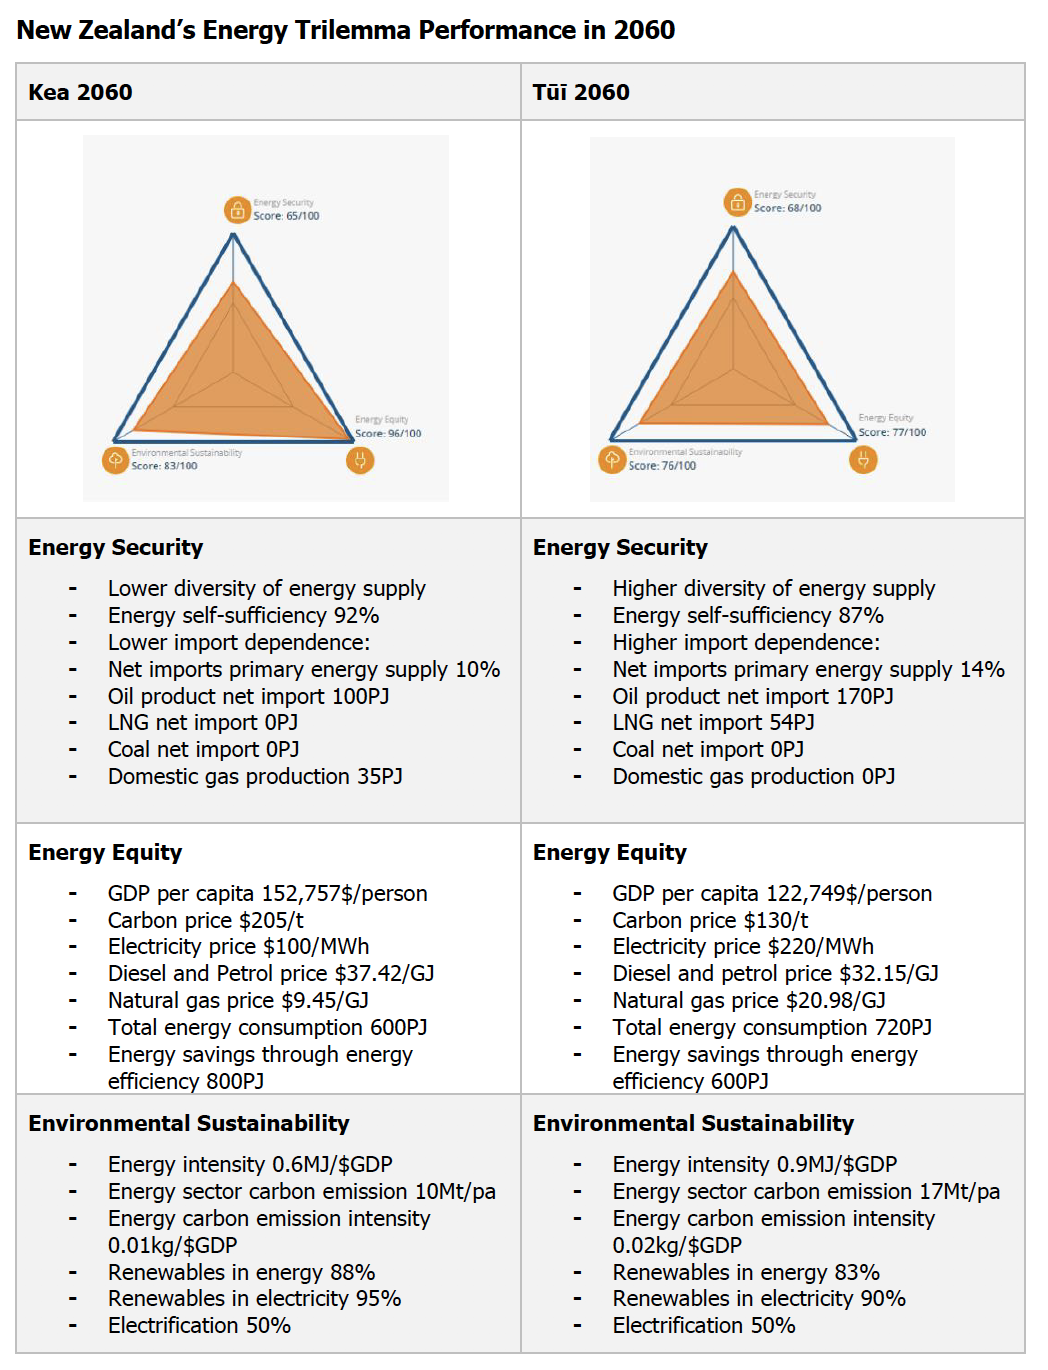
\includegraphics[width=\textwidth]{NZTrilemma}
        \vspace{-1cm}
    \end{center}
    \begin{enumerate}
        \item Analysis of Kayak and Waka
        \item Investigate proliferation of Scenarios
        \item Explorative: Generally explicit about societal and political elements.
        A strong focus on robust input assumptions guiding modelling instead of outcomes.
        \item Focus on techno-economic elements. These are evidence based predictions that aim to
        establish a base case then look at incremental costs and benefits of policies (Conditional Scenarios).
        \item Normative Scenarios: Output driven (UNFCCC or UNSDG Agenda). Backcast to create planning roadmaps.
        \item Explore different scenarios to avoid anchoring bias.
        \item The scenarios help explore New Zealand's Energy Interconnectivity with the rest of the world.
        \item Scenarios allow for more complex growth analysis.
        \item Consider energy demand from Emerging Technologies.
        \item \textbf{Forecast energy demand, technology uptake, to look at relative supply. Cool use of ML possibly}
        \item The inflection point is 2040 to deem if the report is successful or not.
    \end{enumerate}
    There are four critical uncertainties underpinning scenarios due to the number of possible permutations.
    \begin{enumerate}
        \item The way New Zealand - as a society - makes decisions in the future, being either more cohesive or individualistic.
        \item Domestic Acceptance of Climate Change as climate change one of or the most important issue to address.
        \item The level or actual price of carbon compared to the rest of the world.
        \item The degree technology is available to address energy balance and emissions domestically.
    \end{enumerate}
    \begin{center}
        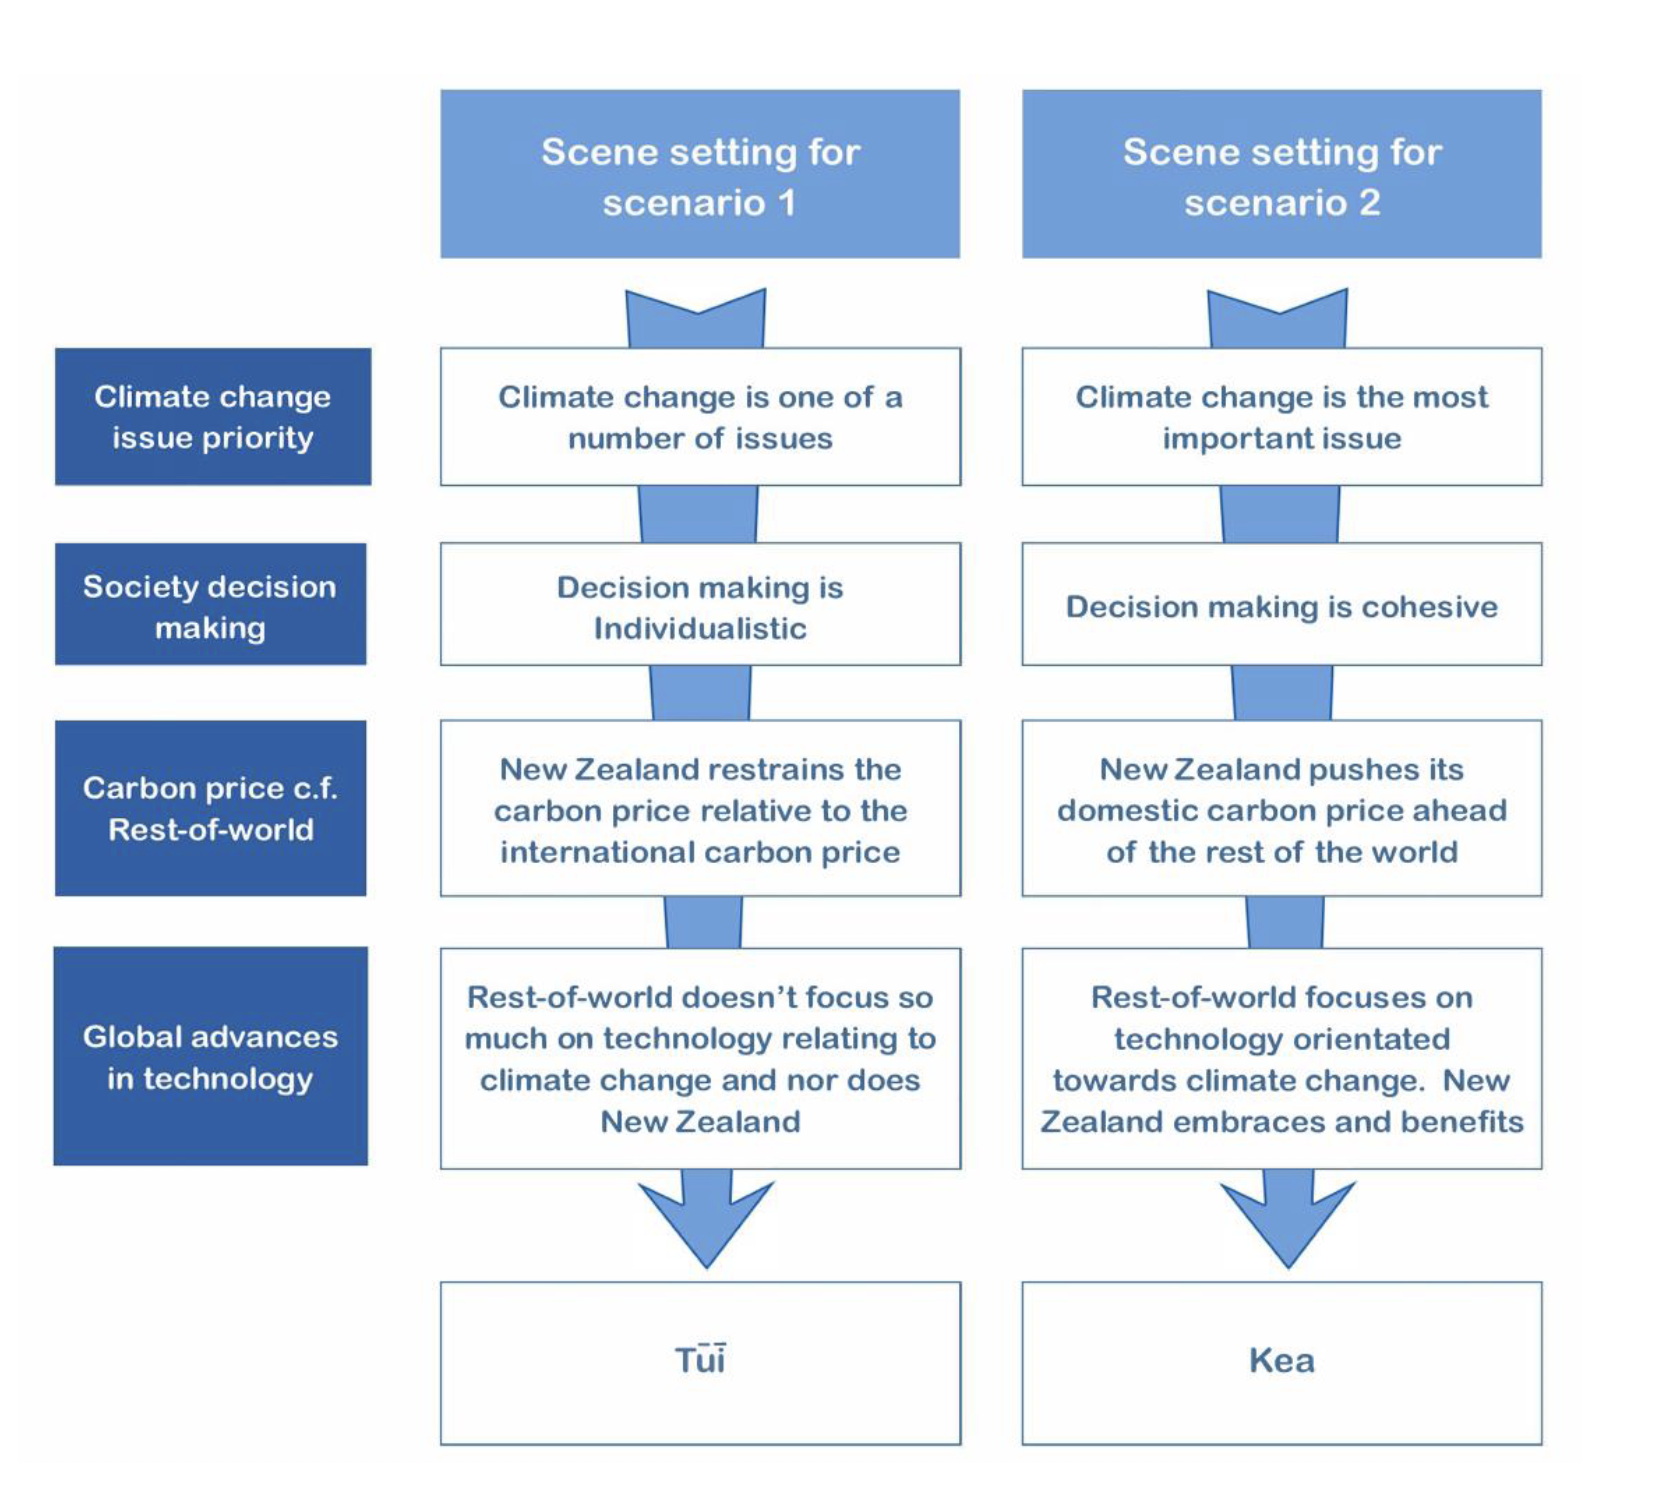
\includegraphics[width=\textwidth]{NZCU}
        \vspace{-1cm}
    \end{center}
    All information relating to the New Zealand Energy Scenarios 2050 is cited from \cite{TR:2}
    \subsection{TIMES Model}
    Modelling the Energy Scenarios Relies on the TIMES Model, an integrated energy-systems model.
    \begin{itemize}
        \item A linear optimisation model, minimising total discounted costs, through time, of meeting all energy service demand.
        \item Simultaneously models all components of an energy system.
        \item Services demanded of the energy system as inputs, not simply forecasts of energy demand. Eg. Vehicles kms travelled or space required for heating.
        \item The model determines which are the optimal technologies to use for the project.
        \item You must forecast services demand.
        \item An array of economic information is produced as a part of the  solution, imforming implied commodity prices
        \item The model has the limitations of a linear model. Maximising the use of a particular technology even if it is only fractionally better than another.
    \end{itemize}
    \begin{center}
        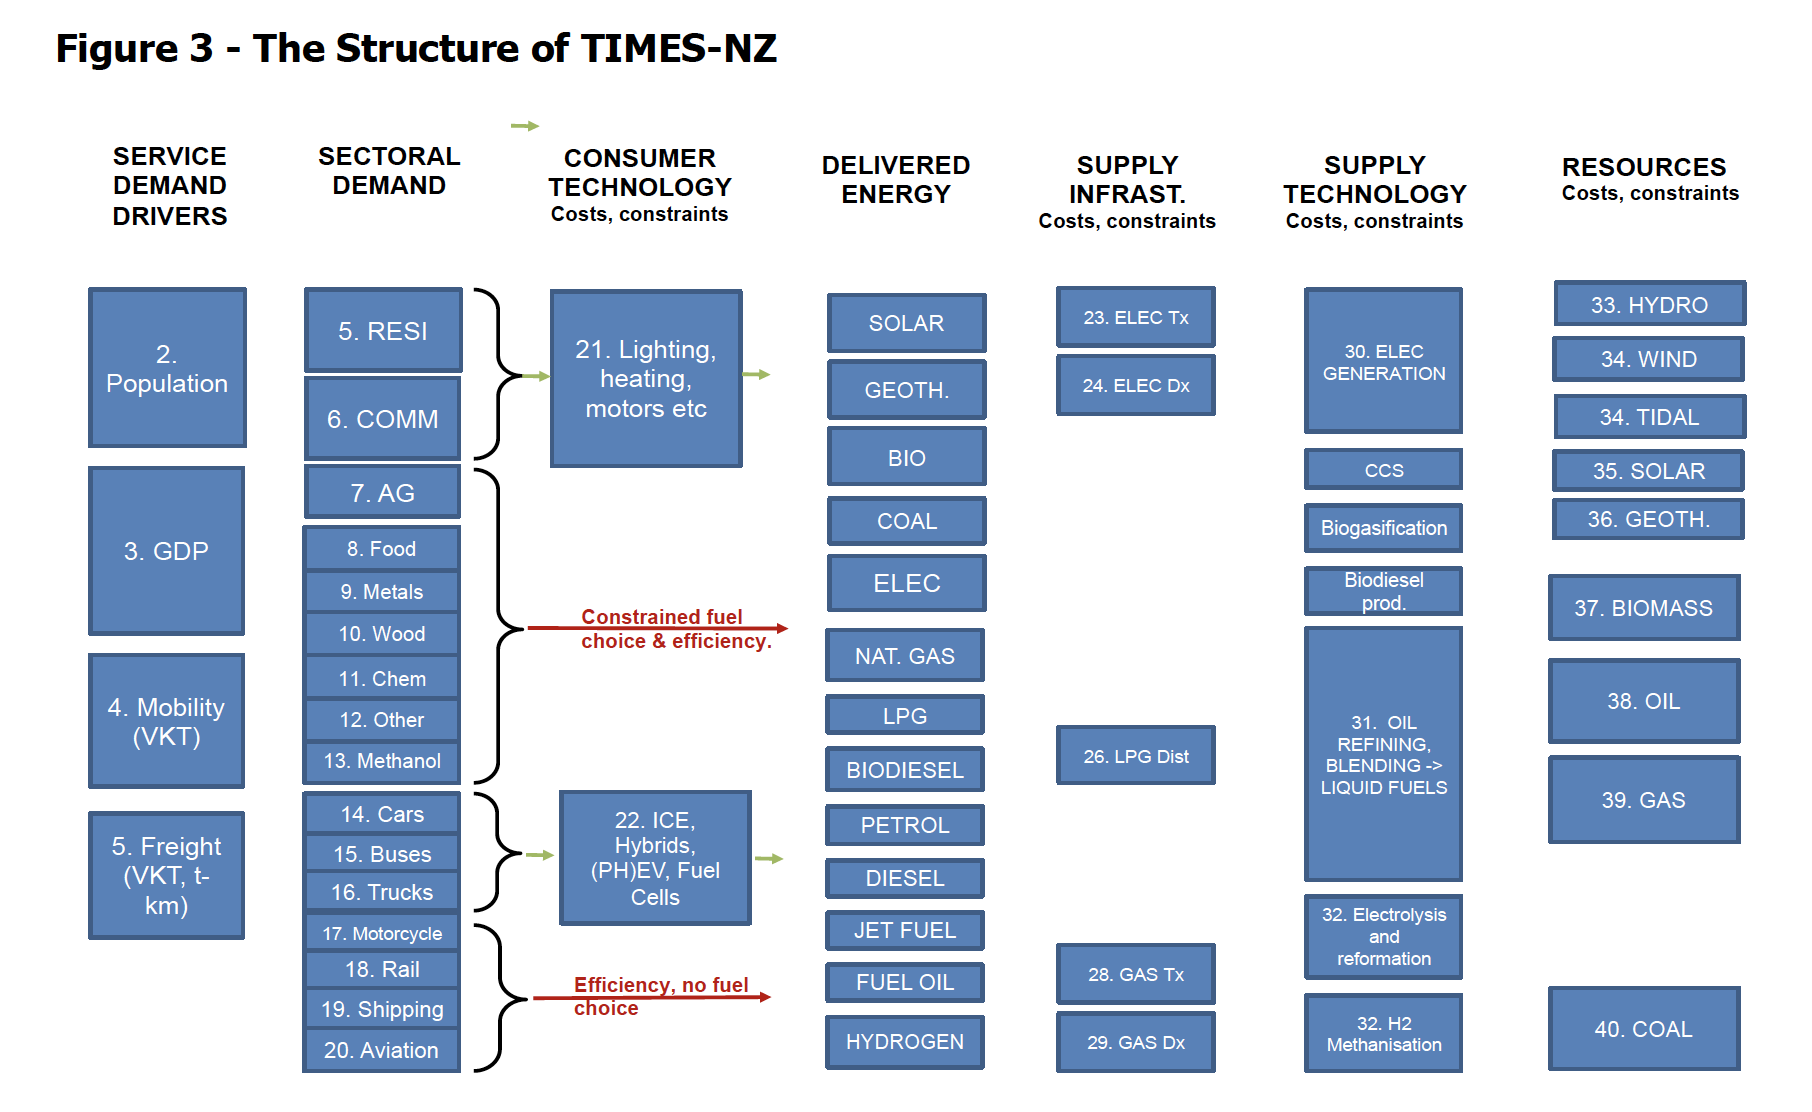
\includegraphics[width=\textwidth]{TNZ}
        \vspace{-1cm}
    \end{center}
    The rest of the report details the impacts both Tui and Kea have on all the relavant economic indicators.
    All information in this section was gathered from 
    \section{World Energy Scenarios 2019 - Full Report}
    \subsection{Key Facts and Summary}
    \section{TIMES Model}
    \subsection{Key Facts and Summary}
    \begin{itemize}
        \item TIMES Model now underpins energy planning around Climate Change and Greenhouse Gas Emissions.
        \item TIMES Model is a bottom up model.
        \item The model can represent an entire economies energy supply chain with Demand, Process and Supply all modelled.
        \item The TIMES model objective is the satisfaction of an exogenous energy service demand at a minimum of total cost over the entire planning horizon.
        \item The model determines the optimal use of fuels and technologies at each period, and the associated trading and emissions activities.
    \end{itemize}
    \subsection{Generalization of the Model}
    \begin{align}
        NPV &= \sum_{r=1}^{R} \sum_{y=YEARS} (1+d_{r,y})^{REFYR-y}\times ANNCOST(r,y)
    \end{align}
    Where:
    \begin{itemize}
        \item NPV = Net Present Value of the Total Costs
        \item ANNCOST = Total Annual Cost
        \item d = General Discount Rate
        \item r = Region
        \item y = Years for which their are costs
        \item REFYR = Reference year for Discounting
        \item YEARS = Set of years there are costs
    \end{itemize}
    TIMES PT uses a partial equilibrium version of TIMES. The actual system encompasses all the steps from primary resources in place
    to the supply of the energy demanded from consumers through all the relevant processes. See another example of the TIMES structure below.
    \begin{center}
        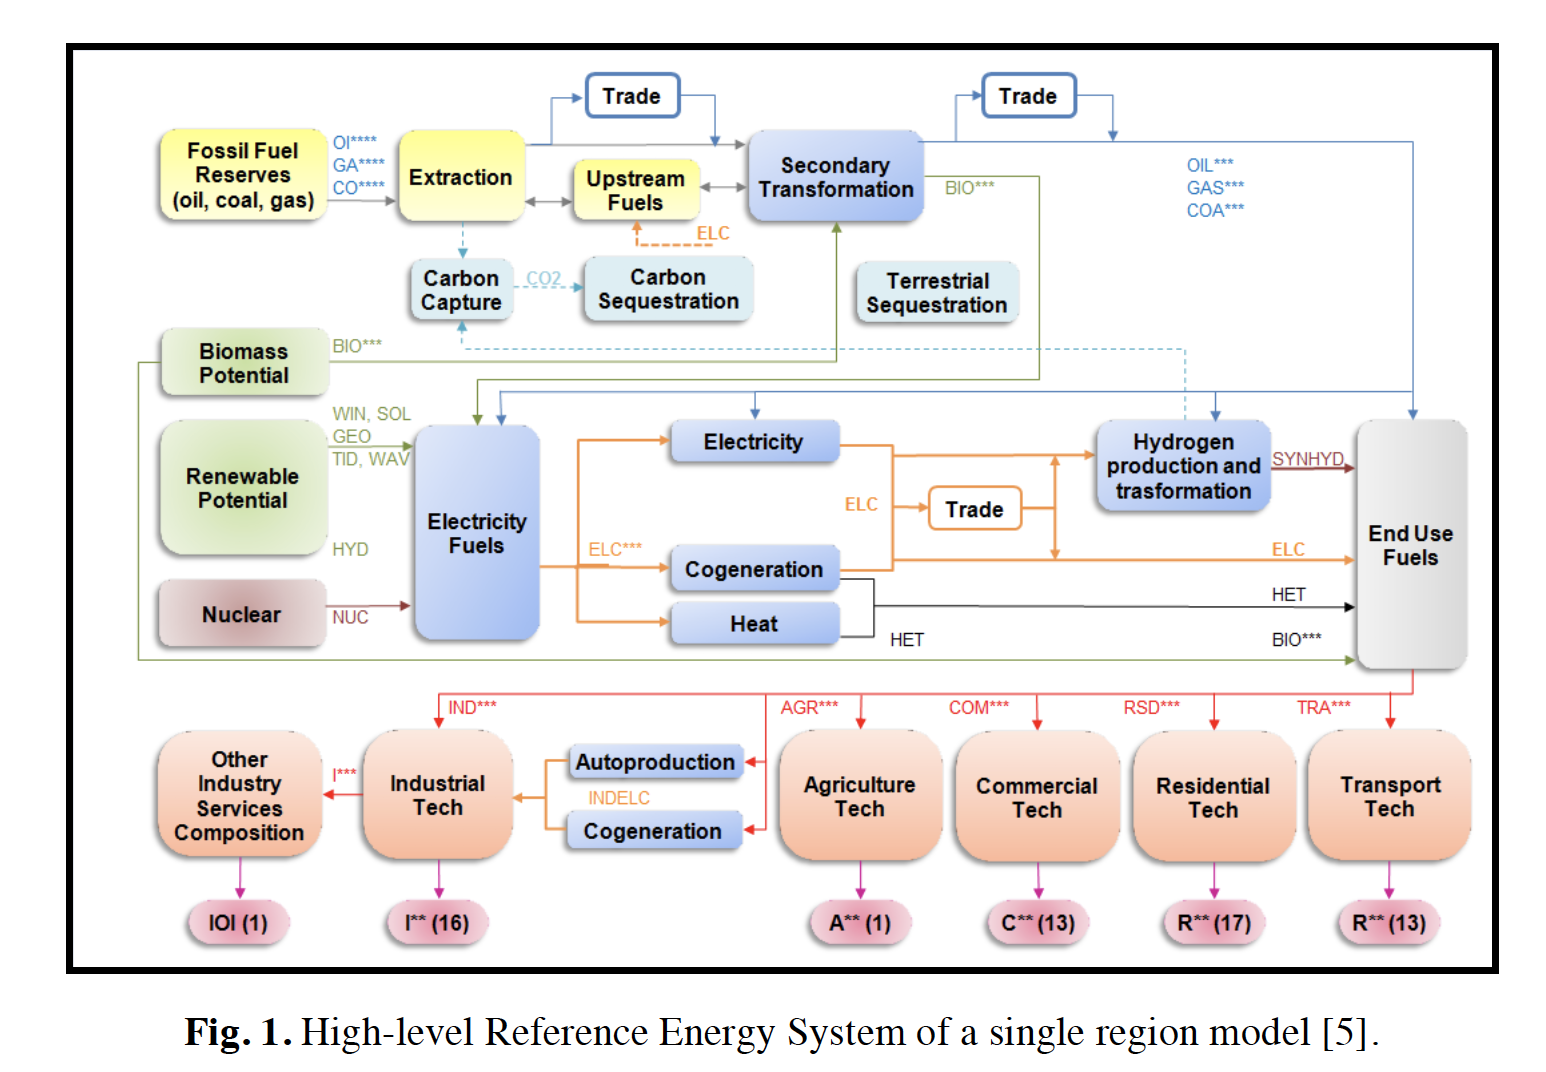
\includegraphics[width=\textwidth]{TIMESPT}
        \vspace{-1cm}
    \end{center}
    \begin{itemize}
        \item Each item characterised by several input parameters of existing and future technologies.
              They are described by means of technical data (capacity,fficiency), environmental emission co-efficients (CO2 etc), 
              and economic values (capital cost, date of commercialisation). Reference demands for energy services and supply curves of 
              the resources help drive drive future developments.
        \item The model is sliced into different sectors: Primary Supply covering Resource Origination, extraction, importing, processing, transport, and distribution.
              each primary resource is modelled independantly, and represented by a linearised stepwise supply function.
              the number of steps approximating each curve depends on the resource and on the country reserves. The energy commodities are disaggregated to the level of detail
              of the extended national energy balances. 
        \item Demand sectors are also represented: In this article, there are 5. 1). Agriculture, 2). Industry, 3). Services, 4). Residential, 5). Transport.
        \item Energy services demand is fed into the model.
        \item Renewable Energy Potential, Primary Energy Prices, Technology Costs and Characteristics. 
              The model combines the technical economic data with energy pricesto dynamically calculate supply cost curves.
        \item There are TIMES technology databases which help forecast trends in technology for the model.
        \item The model can be used for several applications of GHG, air pollutant, and energy scenarios.
    \end{itemize}
    All information in this section was cited from \cite{A:1}
    \section{MARKAL Model}
    \subsection{Key Facts and Summary}
    \section{McKinsey \& Company: The Future is Now: How Oil and Gas Companies can Decarbonise}
    \subsection{Summary and Key Facts}
    \begin{itemize}
        \item Oil and Gas Industry accounts for 9\% of all human made greenhouse gas (GHG) emmissions and produces the fuels that create 33\% of GHG.
        \item Investors are pushing for more active disclosure of Oil and Gas climate policies and plans.
        \item In Australia, New Zealand, Canada, Europe, Japan, and the United States sustainable investments reached assets of \$30.7 trillion in early 2018, one-third of total investment.
        \item Renewables are getting cheaper: The cost of solar - both photovoltaics (PV) and utility scale fallen 70\% since 2011 with the cost of wind by almost two-thirds. By 2025, competitive with Natural Gas.
        \item Still no Global Market for Carbon Taxes
        \item Emissions must be reduced by 3.4 Gigatons of Carbon Dioxide Emissions per Year.
        \item The oil and gas sector must reduce its emissions by at least 3.4 gigatons of carbon-dioxide equivalent a year by 2050, compared with business as usual (90\% reduction). This can be achieved at an average cost of less than \$50 per ton of carbon dioxide equivalent. Process changes and minor adjustments that help companies reduce their energy consumption.
        \item Special initiatives a compnay chooses to reduce its emissions will depend on factors such as geography, asset mix (offshore vs onshore, gas versus oil, upstream versus downstream, and local policies and practises (regulations, carbon pricing, the availability of renewables and the central grid's reliability and proximity)
        \item Companies have already adopted techniques that can substantially decarbonise operations (improved maintenance routines to reduce intermittent flaring and vapour recovery units to reduce methane leaks)
        \item Cutting emissions is not necessary expensive as an offshore operator found that about 40\% of initiatives it identified had a +ve NPV at current prices and an additional 30\% if it imposed an internal carbon price of \$40 per tonne of CO2 in emissions.
        \item Utilisation of Carbon Sinks could help Decarbonisation. \textbf{Potentially use Carbon Taxes to fund carbon sinks in different geographies}.
        \item Plants and trees sequester around 2.4 billion tons of CO2 a year.
        \item Shell offers Dutch customers the opportunity to pay to offset emissions.
        \item The Cost of Carbon Sinks is uncertain as estimates range from \$6 to \$120 per tonne of CO2 in 2030, depending on the source and the sequestration target.
        \item Reducing fugitive emissions and flaring cold contribute 1.5 GtCO2e in annual abatement by 2050, at a cost of less than \$15/tCO2e.
    \end{itemize}
    \begin{center}
        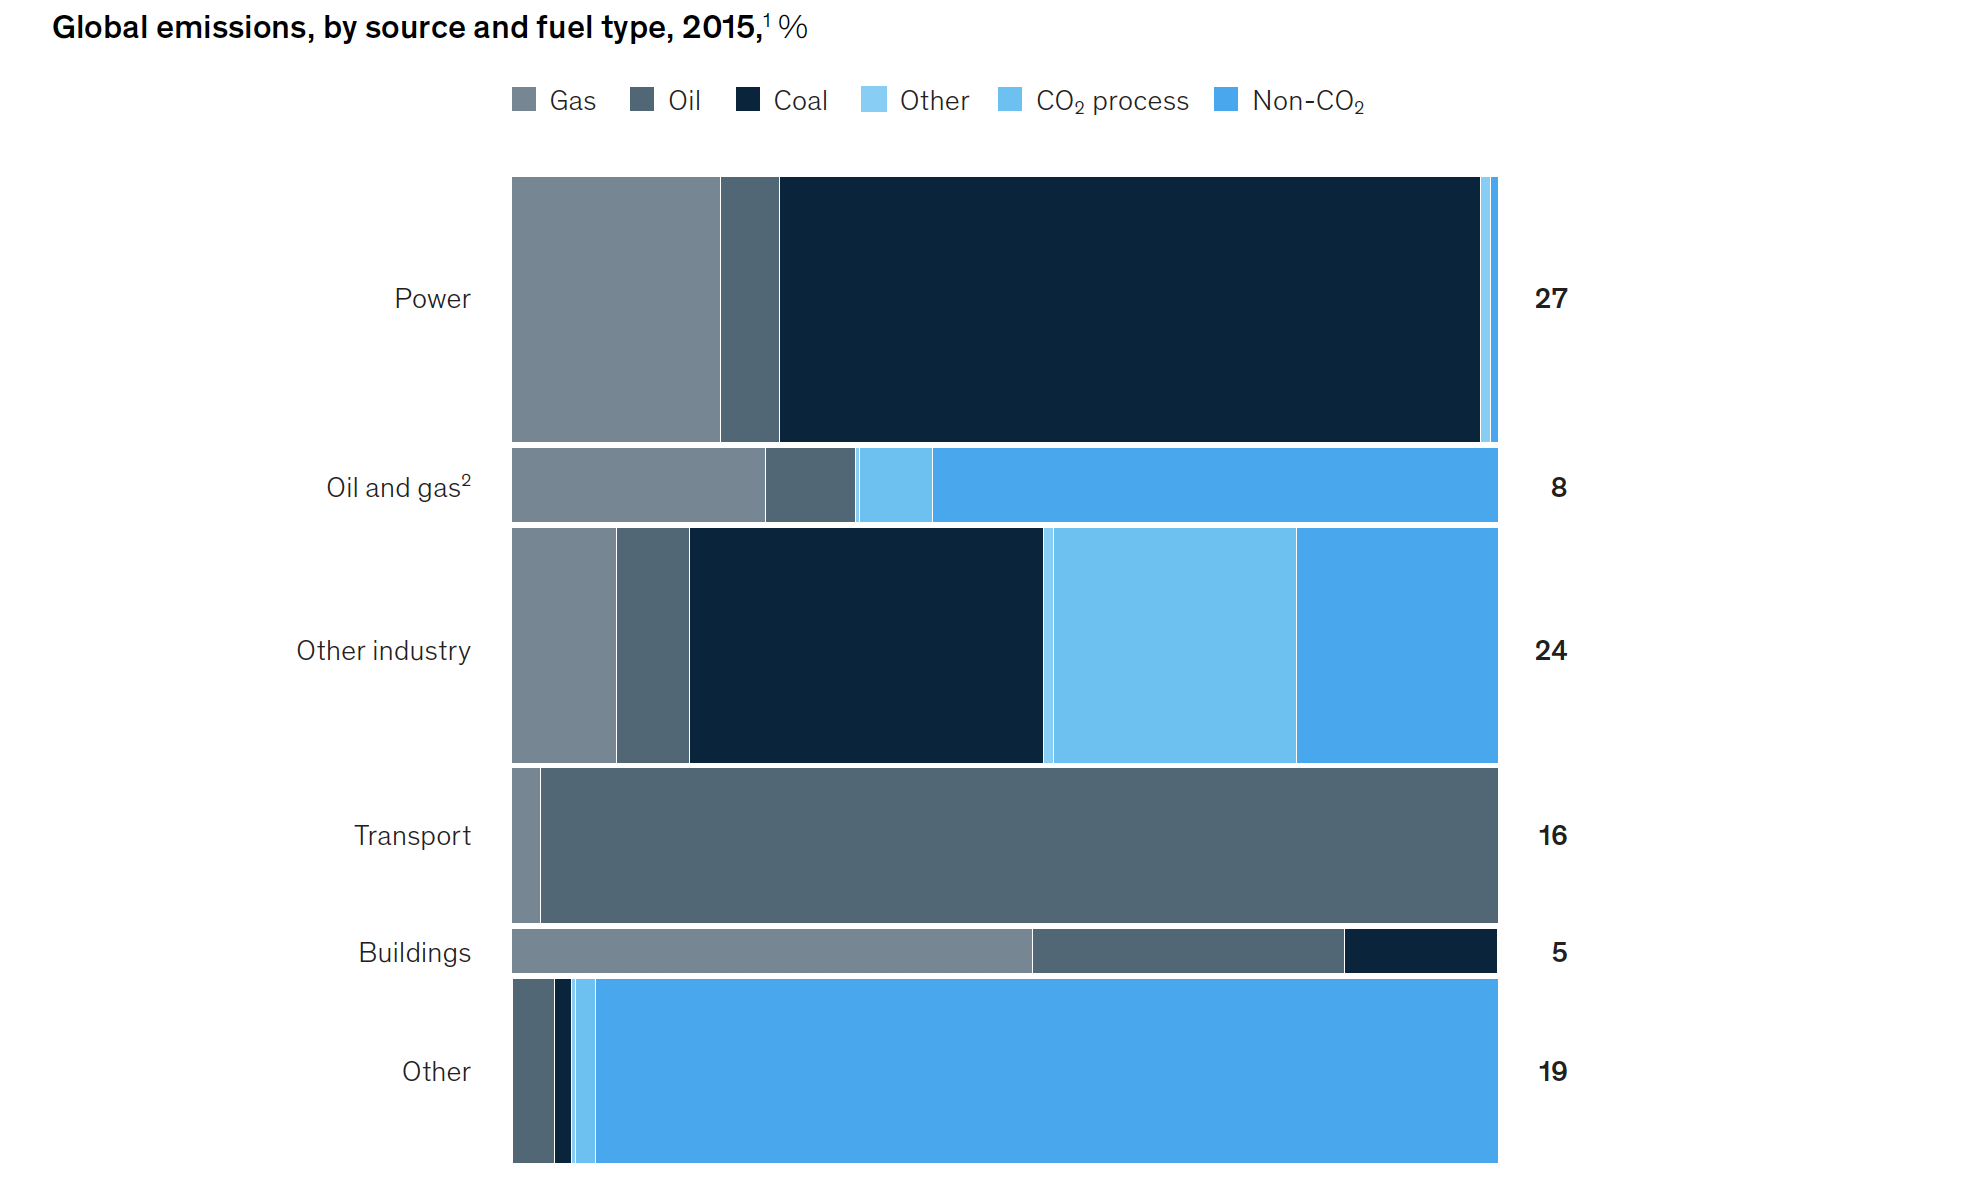
\includegraphics[width=\textwidth]{GE}
        \vspace{-1cm}
    \end{center}
    \begin{center}
        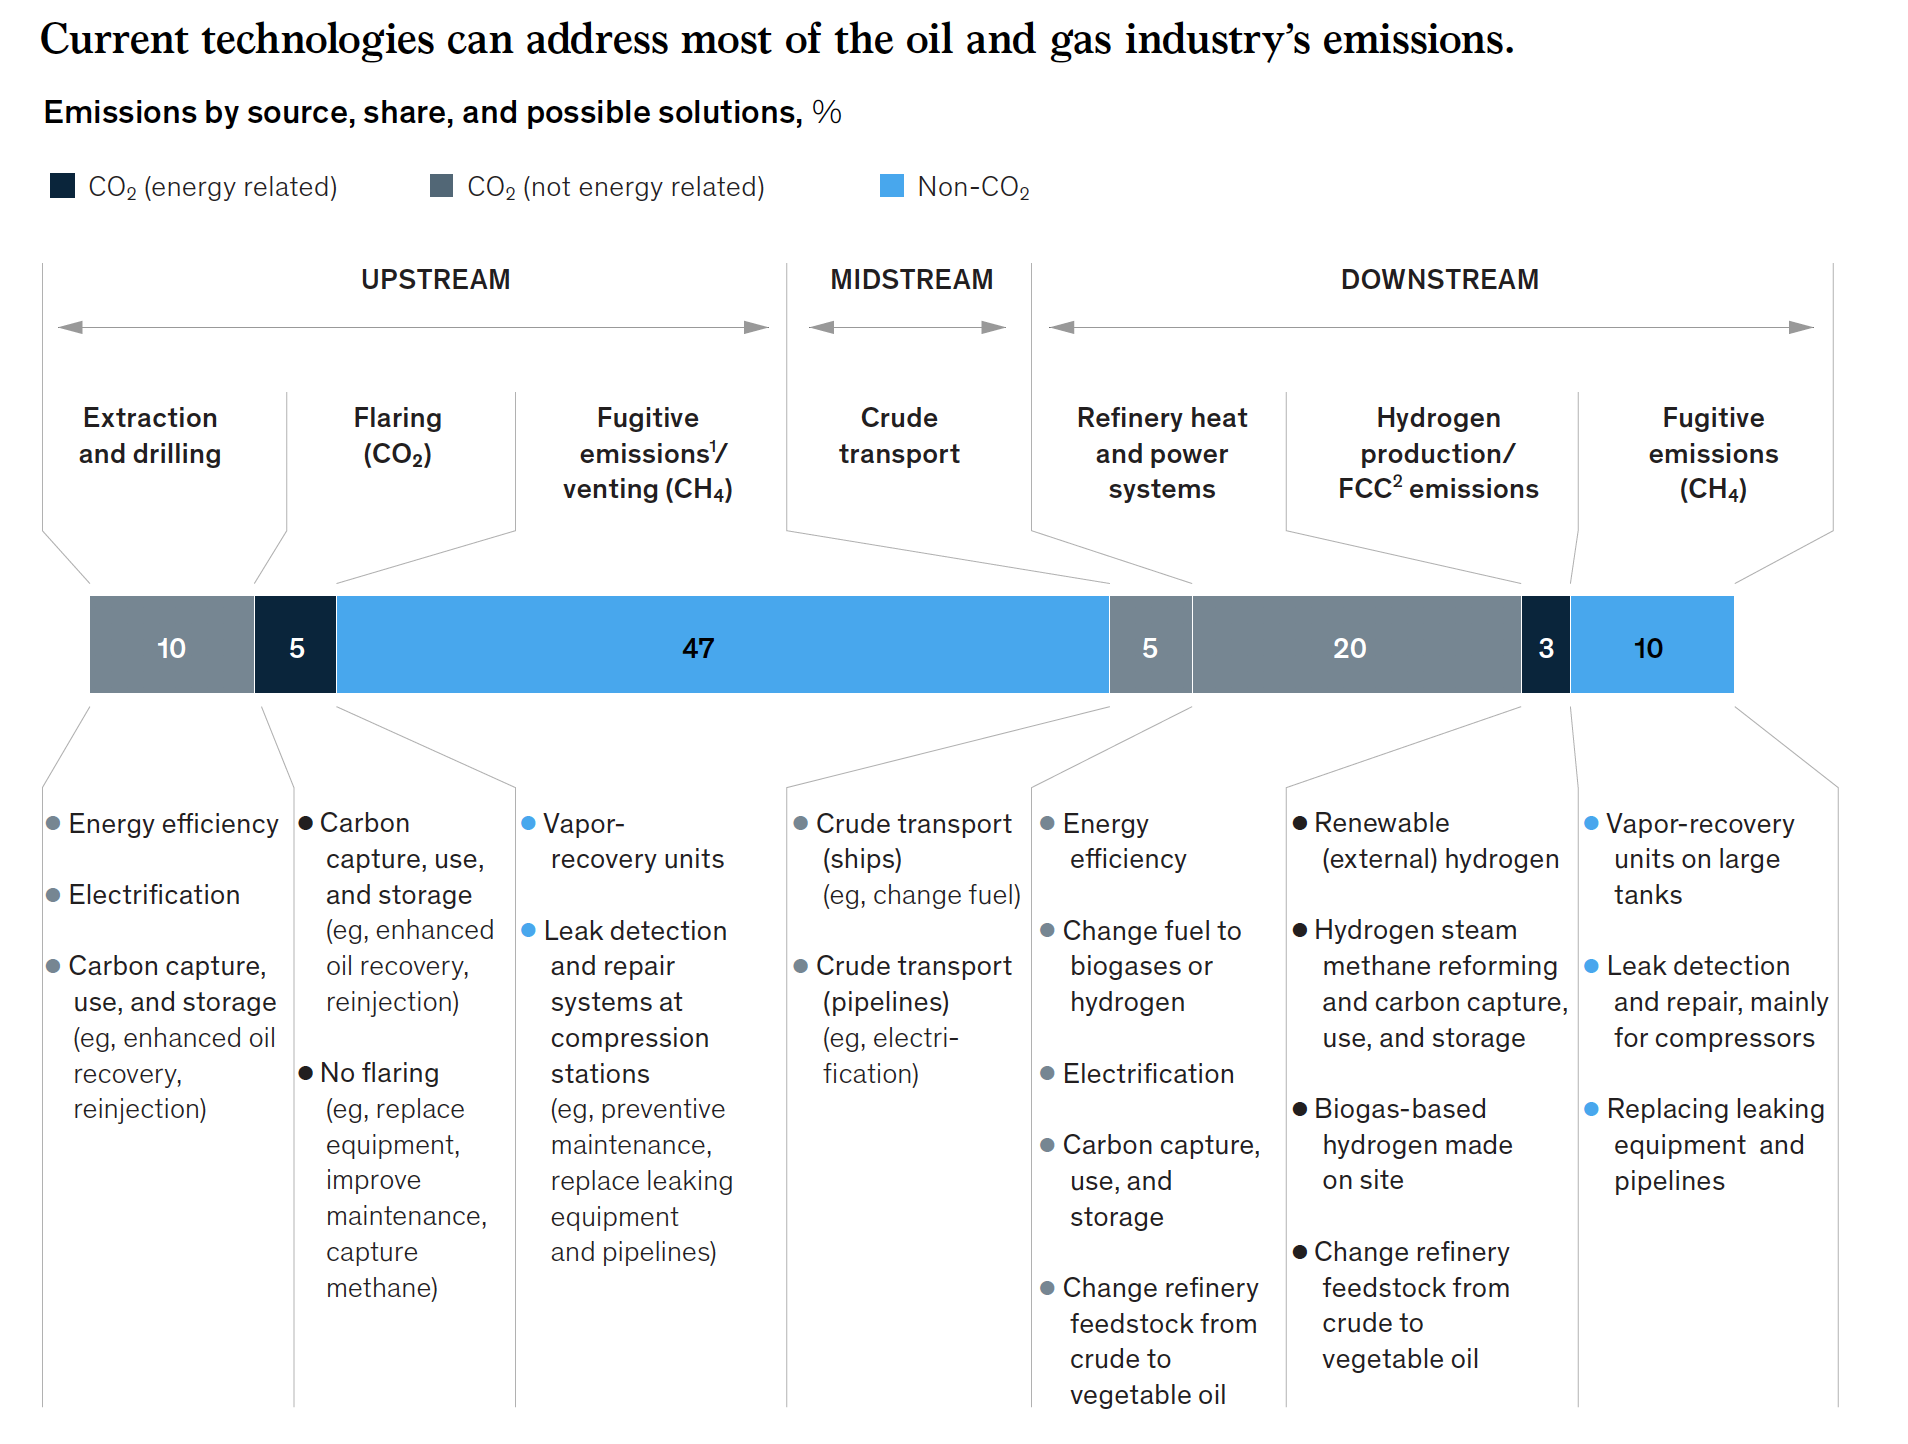
\includegraphics[width=\textwidth]{CT}
        \vspace{-1cm}
    \end{center}
    \subsection{What can Upstream Operators do?}
    \begin{itemize}
        \item Account for two-thirds of sector-specific emissions. Below, we discuss some ways in which oil and gas companies are taking action.
        \item \textbf{Changing power sources}: Use renewable technology to power facilites instead of diesel fuel or fuel gas.
        \item Electrify onshore and offshore operations by connecting to the grid.
        \item Reduce fugitive emissions by applying Leak Detection and Repair (LDAR), installing Vapour-recovery Units (VRU), or applying the best available technology.
        \item Electrifying Equipment
        \item Reducing Non-routine flaring through imprived reliability
        \item Reducing routine flaring through improved additional gas processing and infrastructure.
        \item Increasing carbon capture, use and storage: This technology is projected to play only a minor role i nthe sector's overall decarbonisation.
              O and G there are large scale CCUS facilities in commercial operation, four more are under construction with 19 operating and 28 under development. Total CCUS could increase 200 times from existing 40mtCO2e as CCUS already used for advanced oil recovery.
        \item USA exploring laws and policies to accelerate CCUS development and increasing tax credit.
        \item \textbf{The Clean Gas Project}: A consortium of six oil and gas companies is building what could be the first commercial natural-gas plant with full CCUS capacity.
        \item Rebalancing portfolios: Looking at the composition of upstream portfolio choices. Highest emitting reservoirs (e.g. Complex Reservoirs - highly viscous, in depth or high pressure and temperature may be at a structural emissions disadvantage.)
    \end{itemize}
    \subsubsection{Downstream Operators}
    \begin{itemize}
        \item Energy Efficiency: Waste-Heat Recovery and Medium Temperature Heat Pumps in Refineries.
        \item Green Hydrogen: Hydrogen production through electrolysis has become both more technically advanced and less expensive.
        \item Green Hydrogen is not a speculative technology in oil and gas. Shell and ITM power, a UK-based energy storage and clean-fuel company, are building the world's largests hydrogen electrolysis plant at a German Refinery, with support from the European Union.
        \item Revenue will come from selling hydrogen to the Refinery, which will use it for upgrading its products and for grid balancing payments to the German transmission system.
        \item \textbf{High Temperature Electric Cracking}: Use electric coils instead of fuel gas to provide heat.
        \item \textbf{Use Greener Feedstocks}: Biobased feedstocks or recycled plastic materials (through pyrolysis or gasification).
    \end{itemize}
    Oil and Gas will play an important role in the global energy transition, facing the future is a matter of strategy according to the article. As transparency increases, so may expectations. Customers, employees and investors are already starting to distinguish who are leading the industry.
    All information in this section is cited from \cite{A:2}.
    \section{Pricing Carbon: The Challenges}
    \subsection{Introduction}
    \begin{itemize}
        \item A global carbon tax is to price the externalities caused by greenhouse gas emissions according to the polluter-pays-principle
        \item Politics are a major problem. unpopulr policies lead to denial or procrastination in passing useful legislation.
        \item Lobbyists create significant barriers as can influence politics in a very direct way.
        \item Unilateral action is slow and negotiations have several times coem to a standstill when burden-sharing and fairness are reported.
    \end{itemize}
    \subsection{Carbon Tax}
    \begin{itemize}
        \item The most-cost efficient policy in order to reduce carbon emissions (more so than regulation of technology, products, and behaviours). It affects production levels and consumption levels too.
        \item Carbon Tax encourages the continous reduction of polution rather than Cap and Trade when encourages down to a Cap.
        \item A Carbon Taxes have existed internationally for 25 years. Finland was the first (1990), followed by other Nordic Countries. Only a handle of countries outside
              the nordic countries haver implemented a Carbon Tax of at least \$10 tCO2e to date: (UK, Ireland, Switzerland, and BC in Canada) (More likely in another source)
        \item Sweden's implementation of the Carbon Tax (\$130/tCO2e) has been effective. It applies in particular to transport, where gasoline and diesel are taxed strictly in
              proportion to carbon emissions, but also to commercial use and residential heating as well as partially to industry.
        \item In sweden, ~40\% of final energy consumption comes from Buildings. This heating principle will change on location.
        \item The tax helped phase out fossil fuels for district heating use, switching to recycled and sustainable energy production.
        \item District heating output almost doubled in the district heating sector while carbon emissions dropped 75\%. 
        \item The author says a carbon tax alone is not affective in reducing carbon taxes as their will be a reliance on a combination of instruments with different targets simultaneously.
        \item Sweden saw the economy emissions decrease 9\% while the countries economy experienced a growth of 51\%. There was a strong decoupling between the two.
        \item These figures only took into account products consumed within the country. Greenhouse gas Emissions have decreased by 22\% since 1990 since 1990.
        \item \textbf{A good output metric could be CO2 / GDP}.
    \end{itemize}
    \subsection{Political Challenges with a Carbon Tax}
    \begin{itemize}
        \item In 1990, a political tax failed to be implemented for several reasons. Ministers of Finance were notoriously unwilling to compromise on taxes and give up
              their prerogative on tax issues to supra-national authorities as views as a national convern. They were reluctant on letting the EU decide on yet another area of policy.
    \end{itemize}
    \subsubsection{Global Reasons}
    \begin{enumerate}
        \item Strong lobbying by Fossil Fuel Stakeholders
        \item Opposition from the Public as this raises prices
        \item Transparency as to the effects on winners and losers compared to the much less visible costs of regulation
        \item A perception that taxes reduce welfare and increae unemployment due to lower levels of consumption and production.
        \item Possible institutional path dependencies that led to favouring cap and trade.
    \end{enumerate}
    There were a number of different responses:
    \begin{enumerate}
        \item Removal of Fossil Fuel Subsidies. These subsidies harm the environment in various ways. they also discourage investment in renewable energy and efficiency, and impose a large fiscal burden.
        They can also go towards other public funing initiatives. Inefficient in supporting disadvantaged groups with most of the benefits lying with the rich.
        \item Fuel Consumption: Implement a fuel tax. Fuel has approximately -0.1 to -0.25 price elasticity in ST and -0.7 average in LT.
        \item Cap and Trade, and Regulation: Regulate quantities of emissions and not prices (Advantage for a regulator). Buy/sell excess permits. 
        Permits are allocated either by auction, free allocationm or a mix of both approaches. Revenue is made in auctions but not free allocation.
        \item \textbf{EU Emissions Trading Scheme (ETS)}: World largest CAT programme. (45\% of total GHG Emissions). Emission reductions have been modest. Ironically, 
        the major driver for decreasing global emissions was the financial crisis, not the ETS (COVID-19????). ETS effectiveness compromised due to a latent allocation of permits in the first two phases.
        \item Carbon CAT programmes have been unsuccessful as CAT limits too high woth corresponding low prices to achieve certain reductions. There is heavylobbying to keep industry CAT limits high. CAT has been found to be regressive.
        \item Politicians are worried that a tight cap will hurt their industries. CAT unlikely to work with other policies as move in different directions.
        \item The most contentious part of international negotiations is to link locale schemes without full agreement on targets as no-one wants to lose. Most negotiations focus on an quantative allocation or undertaking by different countries.
        \item \textbf{Promoting Renewable Energy}: New energy infrastructure (from Renewable technologies) is equally important to reducing Carbon Emissions. The price gap in Renewables and Fossil Fuels is quickly decreasing. You can induce renewables to be cheaper than fossil fuels through a carbon tax.
        \item Germnay is a good example of this power transmission. The transition mainly focuses on wind and solar (The most cost-efficient renewable technologies to date)
    \end{enumerate}
    Conclusion
    \begin{itemize}
        \item Carbon Taxe fell politcally out of reach
        \item Cap and Trade - Set to quantity instead of price but difficult to negotiate the cap. India benefit if caps set on a per capita basis while US benefot through grandfathering.
        \item Professors (Academics) should shift focus to prices
        \item Price floors should be implements with quantities, possibly a tax per carbon tonne of carbon. 
        \item Price floor increases global efficiency of carbon mitigation and reduce the risk of leakage and pollution havens, while at the same time the market would receive signals to invest in renewable technologies and emission abatement.
    \end{itemize}
    All information from this section is cited from \cite{A:3}.
\section{References}
\printbibliography
\end{document}
